\section{Trading Environment}

\begin{frame}{Trading Environment}
   \tableofcontents[sectionstyle=show/hide, hideothersubsections]
\begin{center}
  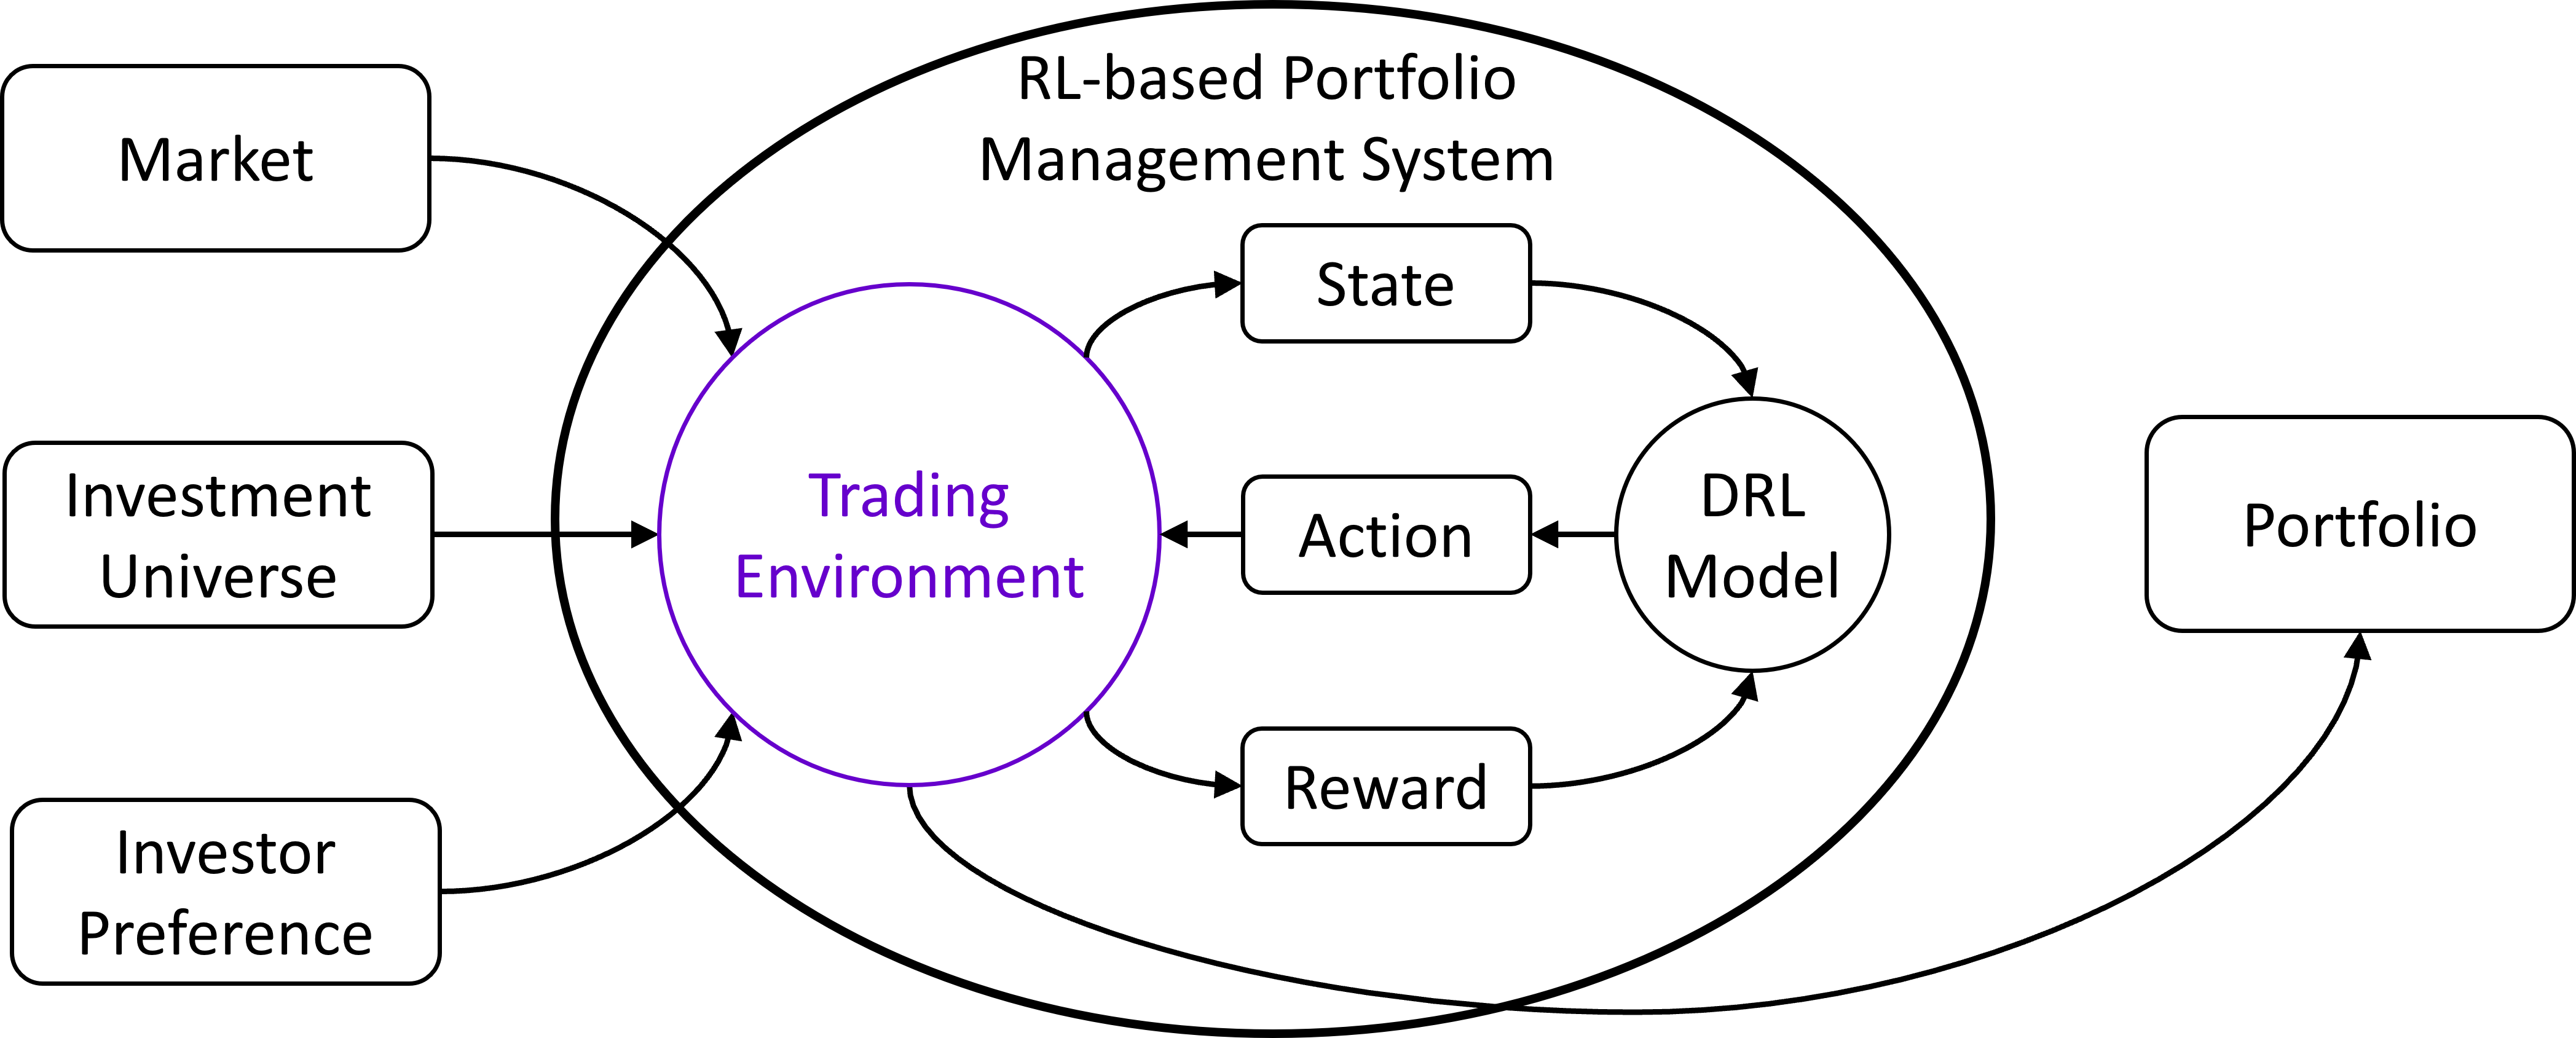
\includegraphics[width=10cm]{images/trading_environment.png}
\end{center}
\end{frame}
\subsection{Feature Extractor}
\begin{frame}{Feature Extractor}
\begin{block}{Objective}
Extract states from the features.
\end{block}
Process
\begin{enumerate}
    \item {
    Normalize the input features}
    \item{Add Gaussian distribution noise to avoid over-fitting}
\end{enumerate}
\alert{Validation results improved significantly after adding noise.}
\begin{center}
  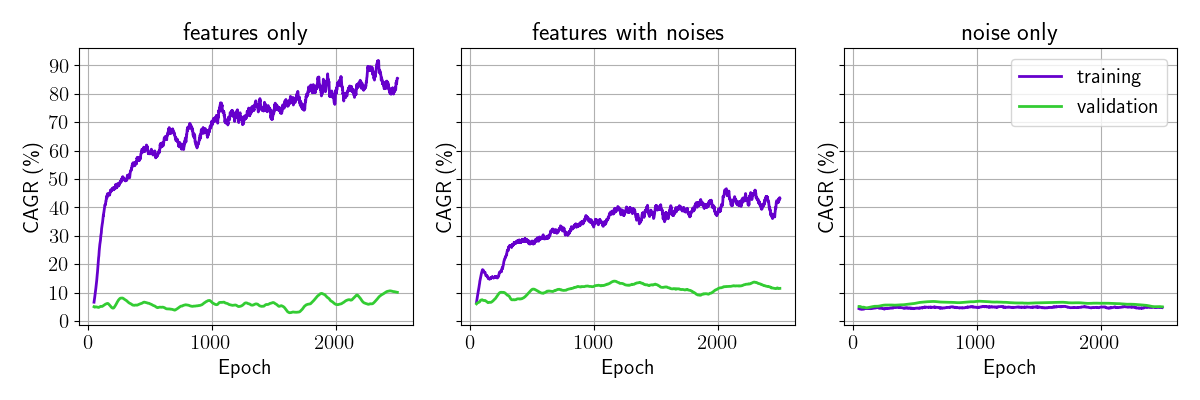
\includegraphics[width=10cm]{images/compare_noise.png}
\end{center}
\end{frame}
\subsection{Portfolio Builder}

\begin{frame}{Portfolio Builder}
\begin{block}{Objective}
Produce the portfoio from action.
\end{block}
\begin{block}{Action}
The action A is a vector space real number between -1 and 1.
\[
    A = \{ {a \in \mathbb{R} } \} ^m,
    a \in \mathbb{R} | -1 \leq a \leq 1 
\]
\end{block}
\begin{block}{Portfolio}
The portfolio F is a vector space of weights f\\
In proportion of normalized action.
\[
    F = \{ {f \in \mathbb{R} } \} ^m,
    {f_i} = \cfrac {a_i+1}{\sum\limits_{i=1}^m {(a_i+1)}}
\]
\end{block}

\end{frame}

\subsection{Reward Provider}
\begin{frame}{Reward Provider}
\begin{block}{Objective}
Provides the reward to the RL model based on the performance of the portfolio and investors preference.
\end{block}
\begin{block}{Option 1: Penalty upon negative profits}
Penalty \(p_t-\theta\), upon negative profits exceeding the threshold \(\theta\). 
\[
p_t = \frac{w_t-w_{t-1}}{w_{t-1}}
, 
R_t = 
\begin{cases}
    p_t,&\text{if  }p_t > -\theta\\
    2p_t - \theta ,&\text{if  }p_t \leq  \theta
\end{cases}
\]
\end{block}
\alert{
\begin{itemize}
    \item Unstable improvement in MDD
    \item Assumption: Optimization goes too well during training and generates a tiny amount of negative profit
\end{itemize}
}

\end{frame}

\begin{frame}{Reward Provider}
\begin{block}{Option 2: Penalty upon both positive and negative profits}
\[
R_t = 
\begin{cases}
    2p_t - \theta,&\text{if  } $$|p_t|$$ > \theta\\
    p_t - \theta ,&\text{if  } $$|p_t|$$\leq  \theta
\end{cases}
\]
\end{block}
\alert{This increases the stability significantly.}
\end{frame}



\begin{frame}{Reward Provider}
\begin{center}
      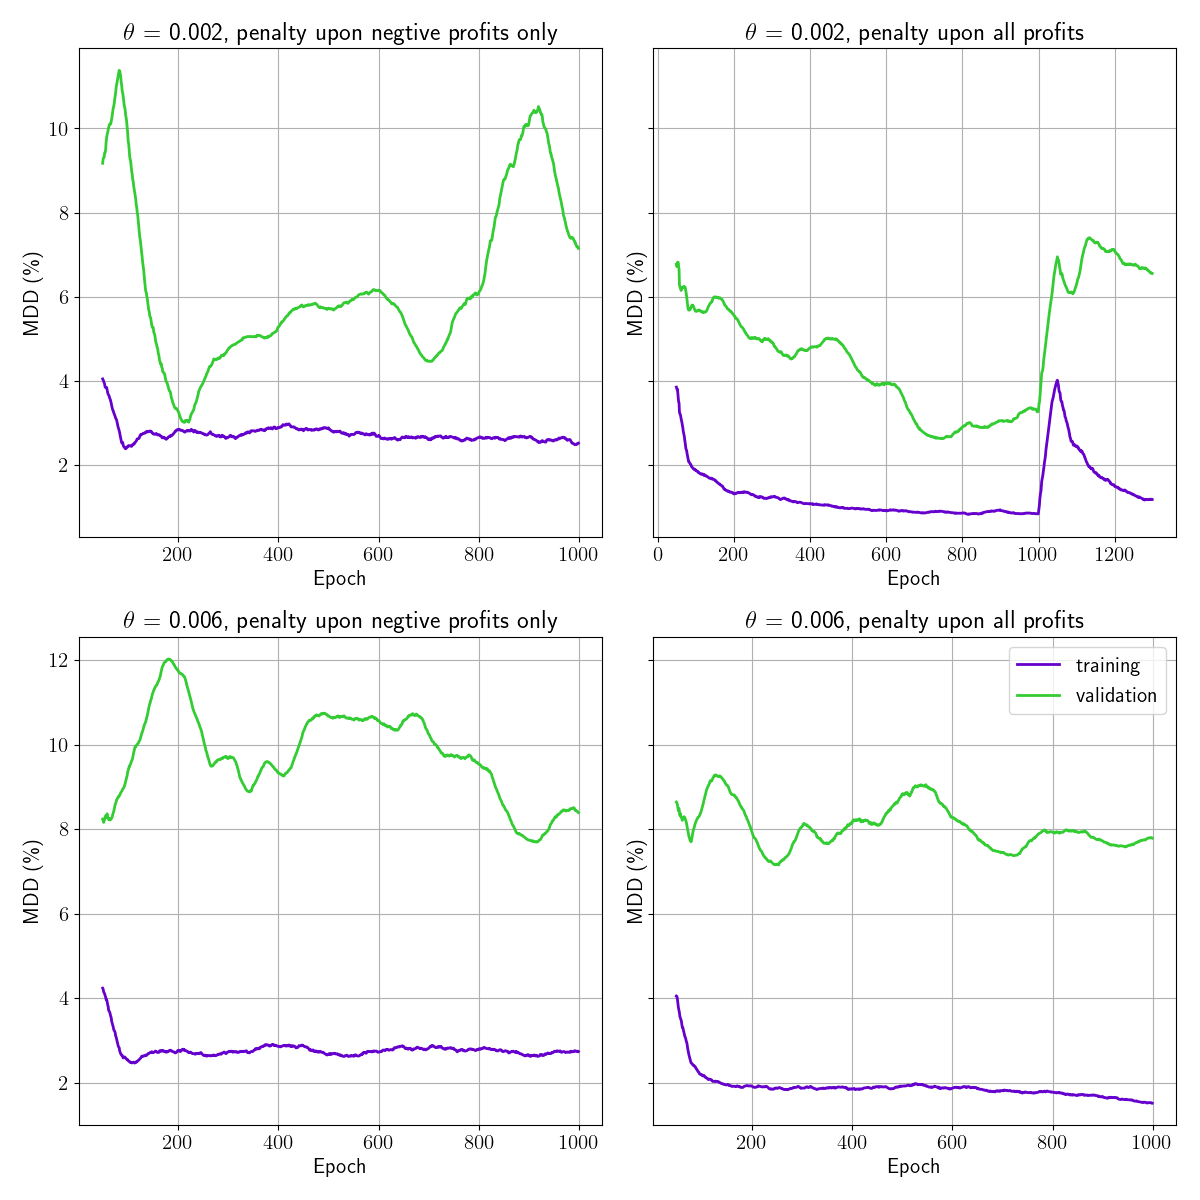
\includegraphics[height=7cm]{images/penalty_negtive_profits_compare.png}
\end{center}
\end{frame}

